\documentclass[conference]{IEEEtran}
\ifCLASSINFOpdf
\else
\fi
\usepackage{graphicx}
\usepackage{amssymb,amsmath,bm}
\usepackage{textcomp}
\usepackage{verbatim} 
\def\vec#1{\ensuremath{\bm{{#1}}}}
\def\mat#1{\vec{#1}}

\begin{document}

\title{Group Delay Functions for Speaker Diarization}

\author{
\IEEEauthorblockN{{ Mohit Yadav, Anil K Sao, A D Dileep and Padmanabhan Rajan}\\
Indian Institute of Technology Mandi\\ 
\  {\small \tt mohit\_yadav@students.iitmandi.ac.in \& \{anil, addileep and
padman\}@iitmandi.ac.in}
}
}

\maketitle


\begin{abstract}

Speaker Diarization is the task of determining {\bf\textit{``who spoke when"}}
in a speech recording of an unknown duration containing an unknown number of
speakers. The very unsupervised nature of this task makes it more challenging
and demanding for the used features to be highly discriminative across speakers.
Popularly used spectrum-related features for speaker diarization take into
account merely the magnitude information and do not utilize phase information
due to the complications involved in its processing. However, the information
embed in phase has been shown beneficial for (mostly supervised) speech tasks,
now it is being explored for speaker diarization. In this work, we propose
group-delay functions based features for speaker diarization. Group-delay
functions are the representations of phase of Fourier spectrum, which overcomes
the issues in processing the phase. We present our experiments and results on a
publicly available meeting corpus. Our experiments demonstrate that the features
derived from group-delay functions provide comparable or improved diraization
accuracy over and on fusion with the popularly used mel-frequency cepstrum
coefficients (MFCC) features. \\

\end{abstract}
\IEEEpeerreviewmaketitle

%\noindent{\bf Index Terms}: Speaker diarization, group-delay functions, all-pole model, agglomerative information-bottleneck.


\section{Introduction}
\label{intro}

Developments in processing power has made possible the digitization of
large-volume spoken documents like news broadcasts, meetings, lectures 
\cite{reviewPaper2,reviewPaper3}. With this digitization, the utility of speaker
diarization systems has increased tremendously because of their applicability to a large 
number of speech applications \cite{reviewPaper1,reviewPaper4}. These applications 
include information retrieval, speech and speaker indexing, 
document content structuring, speaker recognition in presence of multiple or
competing speakers and to help in speech-to-text transcription. Two popular
approaches for speaker diarization are based on hidden Markov models-Gaussian
mixture models (HMM-GMM) \cite{reviewPaper1} and on
the information-bottleneck (IB) principle \cite{aIB2}. In this paper, we focus on the IB principle based approach as it presents a non-parametric solution and also has computational advantages over the
other approach \cite{aIB2}.

%\subsection{Related Work}
In recent years, the scientific community has seen significant amount of work on
improving features for diarization systems. Broadly this work can be divided
into three categories: (a) spatial information fusion, (b) 
robust overlapped speech handling and (c) learning-based features. Spatial
information fusion based methods exploit multiple recordings acquired using a microphone array often 
referred as multiple-distance-microphones (MDM) \cite{aIB3,aIB4,featAngle,speakerUPM,featSpatial,MDM}. 
These methods enjoy the resultant spatial redundancy, and claim to provide complementary features to
conventionally used MFCC features \cite{MDM}. On the other hand, the approaches from the other two categories do not make any explicit use of spatial information arising from MDM. However, these approaches do make use of multiple recordings implicitly by utilizing one single enhanced recording obtained after beamforming multiple recordings obtained from MDM \cite{beamforming}.

The next category of methods are motivated by fact that the effective handling of
overlapped speech is considered to be at the limits of the current 
state-of-the-art of speaker diarization systems \cite{reviewPaper1,featOverLap}. In the same
spirit, authors in \cite{featProsody,featOverLap} have explored long-term
conversational and prosodic features to detect and handle overlapped speech more
robustly. Next in \cite{featSC}, authors have utilized features based on a convolutive non-negative sparse-coding approach to further improve the detection and handling mechanism for overlap speech. 


The last category of approaches advocate the use of features
obtained by applying learning-based methods. Authors in \cite{featANN}, have
proposed an artificial neural network-based based approach to learn a feature transform,
aimed to distinguish segments from different speakers. Similarly, authors in
\cite{featPCAnLDA} utilize traditional principal component analysis (PCA) and
linear discriminant analysis (LDA) to perform feature selection, at the initial
and the final stages of diarization respectively. With an exception to
above mentioned categories, authors in \cite{featFilterBank}, have derived
features using filter-bank-slope of the magnitude spectrum, and attributed their success to their ability to emphasize formant structure present in the spectrum. 

Feature derived from magnitude spectrum such as MFCC are ubiquitously used in various
speech tasks. On the other hand, use of the phase of short-term spectrum is not so
widespread, due to the difficulties in its processing.
However, there has been a significant increase in the interest to utilize
information from the phase spectrum recently
\cite{phaseImportantInterspeech14,gdSurvey}. Traditionally, \textit{group delay functions}
and their variants have been used to mitigate difficulties involved in
processing the phase. Features derived from
group delay functions have shown promise for other speech tasks, and here we 
explore it for speaker diarization \cite{modifiedGD,allPoleGdSid}. 

In this work, we propose features derived from group delay functions for
IB based speaker diarization. The primary objective
is to investigate whether group delay based features can be used
effectively in the context of speaker diarization and if they can supplement magnitude-based
features. The layout for the remaining paper is as follows: section \ref{fe} introduces
group delay functions and difficulties involved in their
processing. Subsequently, section \ref{system} discusses the used IB-based diarization
system briefly. Next in section \ref{feature_analysis_and_fusion}, we present the performed comparative and fusion analysis on the features derived from group delay functions. Their performance is evaluated using publicly AMI meeting corpus (\cite{AMIData}), in context of the introduced diarization system in section \ref{experimentsNresults}. Lastly, section \ref{conclude} provides conclusion and directions for future work.    

\section{Group delay functions}
\label{fe}
Let us denote a frame of speech as $x(n)$ and its Fourier transform as
$X(\omega)$. The polar representation of $X(\omega)$ can be written as follows:

\begin{equation}
X(\omega) = |X(\omega)| e^{j\theta(\omega)} 
\label{equ:FT}
\end{equation}     
where $|X(\omega)|$ and $\theta(\omega)$ refers to magnitude and phase part of
the spectrum respectively. The group delay function is defined as the
negative derivative of the continuous (i.~e.~unwrapped) phase of Fourier transform, and can be written
as follows: 
\begin{equation}
\tau(\omega) =  - \frac{d}{d\omega} \theta(\omega).
\label{equ:GDF_def}
\end{equation}

The high-resolution and additive properties of group delay functions have been
studied earlier (\cite{yegnaJASA, gdSurvey}). As a result of this, in the
group delay domain, very closely
spaced spectral peaks (or valleys) are confined to narrow regions around poles
(or zeros.) However, computation of unwrapped phase of Fourier transform is a
non-trivial task. To bypass this, the group delay function can be computed
directly from the speech signal, without phase unwrapping, as
\cite{gdDerivationIcassp}:

\begin{equation}
\tau(\omega) = \frac{X_R(\omega)Y_R(\omega) +
X_I(\omega)Y_I(\omega)}{|X(\omega)|^{2}},
\label{eq:GDF_com}
\end{equation}

where $y(n) = n x(n)$, and $Y(\omega)$ is its Fourier transform. 
Subscripts $R$ and $I$ in equation \ref{eq:GDF_com}, represents real and
imaginary part of Fourier transform respectively. 

The proximity of a zero (spectral dip) near the
unit circle results in a very small value of the denominator in
equation \ref{eq:GDF_com}. This results in spikes of large magntide in the group
delay spectrum. As a result, the formant information present in the group delay
spectrum is masked. More details about the behaviour of group delay functions
can be found in \cite{gdSurvey}.

To address the above mentioned issues, the
\textit{modified group delay function} (MODGDF) has been proposed
\cite{modifiedGD}, which can
computed using the following expression:
\begin{equation}
\tau_{m}(\omega) =  
\frac{X_R(\omega)Y_R(\omega) + X_I(\omega)Y_I(\omega)}{|S(\omega)|^2}, 
\label{eq:MODGDF}
\end{equation}
where, $|S(\omega)|$ is obtained from $|X(\omega)|$ by cepstral smoothing.
Features derived from the modified group delay function have been used in
several speech tasks \cite{modifiedGD}.
%And parameters $\alpha:(0,1]$ and
%$\gamma:(0,1]$ are used to control its dynamic range. Again, subscripts $R$ and
%$I$, represent real and imaginary part of Fourier transform respectively. 
Another method to overcome the limitations of equation \ref{eq:GDF_com} is to
derive the group delay function from an all-pole model. Such a parametric
representation of group delay functions was first described in \cite{yegnaJASA}.
The parametric model used is
\begin{equation}
H(\omega) =  \frac{G}{1 - \sum_{k=1}^{k = p} a_k e^{-j\omega k}}.
\label{eq:homega}
\end{equation}
Here, $p$ is the model order, and the gain factor $G$ is set to unity. The model
parameters $a_k$ are estimated by solving the standard Yule-Walker equations. As
the filter contains only poles, the spectrum $H(\omega)$ will not have any
zeros.  Computing the group delay function from the phase spectrum of
$H(\omega)$ will not result in spurious peaks, as in equation \ref{eq:GDF_com}.
The resulting filter is minimum-phase, and thus the spectrum $H(\omega)$ in
equation \ref{eq:homega} has some information loss when compared to the signal
spectrum $X(\omega)$. Features derived from the all-pole group delay function
have been used earlier for speaker recognition \cite{allPoleGdSid}.

\section{Information-bottleneck based diarization}
\label{system}

%{\{c_1,c_2,..,c_K\}}

Information bottleneck (IB) based diarization is studied in
\cite{deepuThesis}. The underlying principle is to represent the data $X$ as a
set of clusters $C$, usually with $|X|>|C|$. The distortion between $X$ and $C$
is attempted to made minimum. A set of relevance variables $Y$ is used to
determine the set of clusters $C$. In general, $Y$ represents some meaningful
representation of the information present in $X$ (in other words, the relevant
information present in $X$.) In information theoretic terms, the set $C$ 
should maximize $I(Y,C)$ constrained by
$I(X,C)$, where $I$ represents the mutual information. This can be achieved by
maximization of the below criterion:
\begin{equation}
\label{eq:aIB}
F = I(Y,C) - \frac{1}{\beta}I(X,C) 
\end{equation}
where $\beta$ is the Lagrange multiplier which represents the tradeoff between
the information preserved $I(Y,C)$, and the compression achieved $I(X,C)$
\cite{deepuThesis}. The choice of $Y$ can vary with the underlying
application. The IB principle also assumes that the conditional distribution
$p(y|x)$ is also available (or can be estimated.)

When applied to speaker diarization, the input variables $X$ are sequences of
short-time features extracted from speech frames. $X$ corresponds to a uniformly
segmented (typically of length 2.5 seconds) sequence of feature vectors. The
relevance variables $Y$ refer to the components of a Gaussian mixture model in
the feature vector space, learnt from the entire input speech recording. The GMM is
estimated with a shared covariance matrix, and the number of components are
dependent on the number of segments (described earlier) in the input utterance.
The conditional probability density $p(y_i|x_j)$ can be estimated by determining
the contribution of the $i$th GMM component to the $j$th speech segment
\cite{deepuThesis}.

The agglomerative IB (aIB) based diaraization is described as follows. At initial stage, each segment $X$ is
considered as a separate cluster. Subsequently, segments are iteratively merged such that 
at each iteration, the decrease in the goodness of representation (determined using 
equation \ref{eq:aIB}) of the current set of clusters $C$ is least. The number of 
clusters is determined using an empirically learned threshold on normalized mutual 
information, i.e., $\frac{I(Y,C)}{I(Y,X)}$. This represents the 
fraction of the original mutual information that is captured by the current cluster
representation, and monotonically decreases with the number of clusters.  The
normalized mutual information will decrease rapidly when more dissimilar clusters are merged. The
algorithm finally refines the initial uniform segmentation be performing a
Viterbi realignment. More details of the algorithm (termed as aIB algorithm)
can be found in \cite{deepuThesis}.

%\begin{comment}

\section{Feature Analysis}
\label{feature_analysis_and_fusion}
In order to show the effectiveness of group delay-based features, analysis is performed in following two parts: comparison and fusion analysis, as explained below in section \ref{feature_analysis} and \ref{feature_fusion} respectively. The objective behind the former part of the analysis is to compare the ability of group delay-based features with MFCC features, to capture the speaker information in context of speaker diarization. And the latter part of the analysis is intended to test whether group delay-based features on fusion with MFCC can boost up the overall performance of the speaker diarization system. 
 
%\subsection{MFCC v/s Group-delay based features}
\subsection{Comparison : MFCC and group delay-based features}
\label{feature_analysis}

We analyse speech-segments created prior to applying aIB algorithm arising from the input variable $X$. Each speech-segment is modelled using a Gaussian distribution and the covariance matrix is shared across all speech-segments present in the entire speech recording \cite{featFilterBank}). Speech-segments are than divided into two set of pairs, namely, inter-speaker and intra-speaker, based on the available ground-truth label information. Then Kullback-Leibler Divergence (KLD) between the pairs of speech-segments is computed for both the sets \cite{kld}. The mean and variance of KLD computed on randomly selected $20$ speech recordings, are reported in Table \ref{table:kl-div}. 

\begin{figure}[h]
\centering
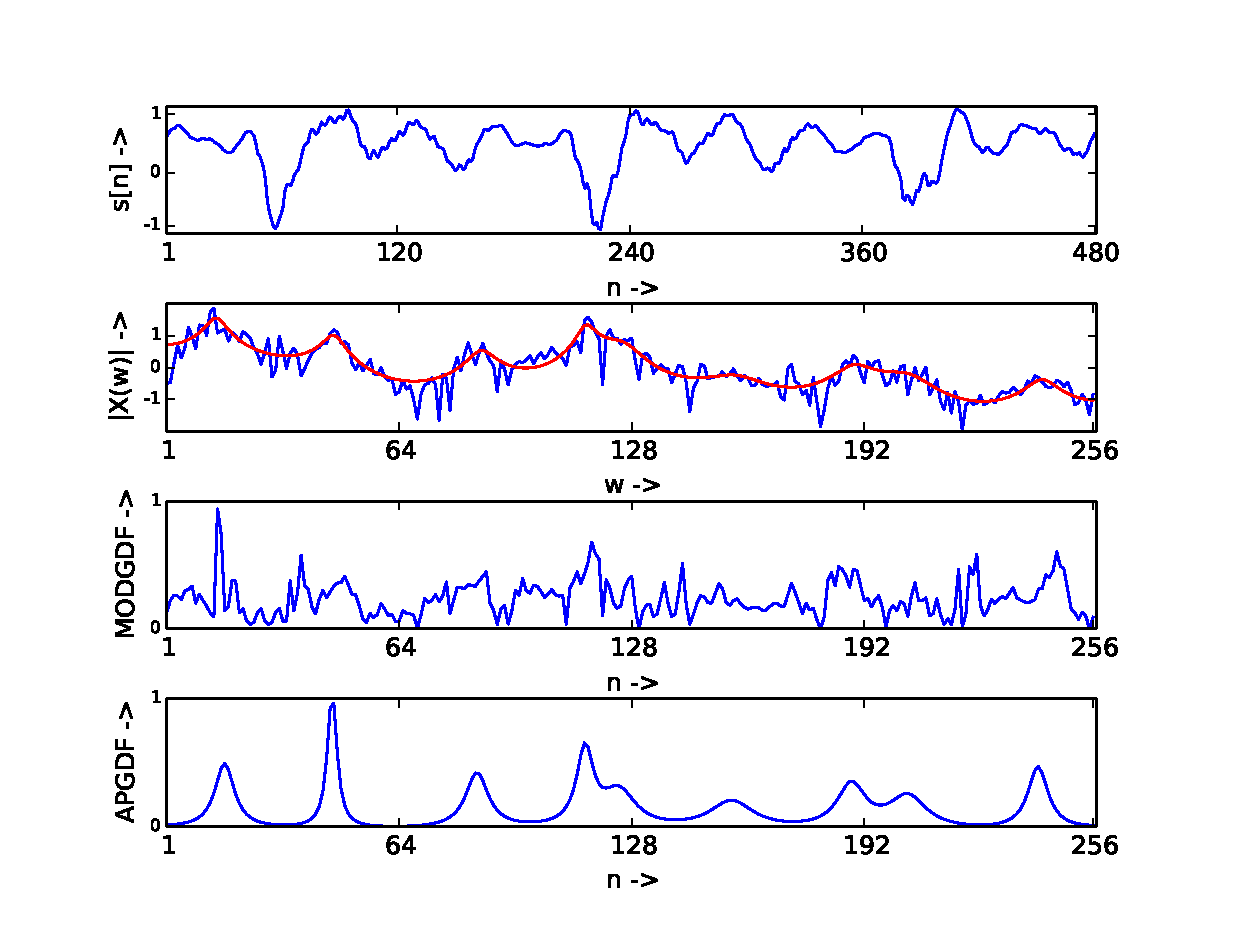
\includegraphics[width=0.5\textwidth,height=10cm]{figures/apSpectrum.eps}
\caption{ A frame of speech (in the top panel), corresponding magnitude of
Fourier spectrum(DFT) and its approximation by all-pole model (in the second
panel), modified group-delay function (in third panel) and group delay function 
based on all pole model (in the bottom panel).}
\label{fig:all-pole}
\end{figure}
%\end{comment}


\begin{table}[h]
\centering

\label{table:kl-div}
\begin{tabular}{|l|l|l|}
\hline
Feature 			& Intra-speaker 			& Inter-speaker 	 \\ \hline
MFCC          			& 6.7/10.1               & 8.3/11.4       \\ \hline
MODGDF        			& 6.1/9.7                & 8.4/12.7       \\ \hline
APGDF         			& 5.5/9.7                & 8.6/11.9        \\ \hline
\end{tabular}

\vspace{0.4cm}
\caption{KL divergence for both inter-speaker and intra-speaker speech segments
created at to initialize the aIB algorithm.}
\end{table}

The decrease (increase) in the mean of KLD value for intra-speaker (inter-speaker) set for 
both MODGDF and APGDF suggests that group delay-based feature can capture speaker
information in context of IB based diarization systems. Additionally, the variance of KLD value for intra-speaker (inter-speaker) set has decreased (increased) which further indicates the better separability achieved by group delay-based features when compared with MFCC features. 

\subsection{Fusion : MFCC with group delay-based features}
\label{feature_fusion}
As explained earlier in section \ref{system}, the IB based diarization requires the following: a) the input variable $X$, b) the relevance variable $Y$, and c) the conditional distribution $p(y_i|x_j)$ (as defined above). For example, features to fuse are $m$, and $g$, then input variable $X$ is a trivial fusion of $j^{th}$ speech-segment across features, i.e., $x_j = \{x^{m}_j,x^{g}_j\}$, as the initial segmentation is shared across feature streams. To estimate joint relevance variable (i.e., $y_i = \{ y_i^{m},y_i^{g}\}$), two separate GMMs are learnt for $m$, and $g$ such that, $y_i^{m}$ and $y_i^{g}$ component of GMMs are estimated using $x^{m}_i$ and $x^{g}_i$ ($i^{th}$ speech-segments of the corresponding feature streams) respectively. One to one relationship between components of GMMs across feature streams allows to estimate the conditional probability density $p(y_i|x_j)$ for fusion of two feature streams as follows:

\begin{equation}
p(y_i|x^{m}_j,x^{g}_j) =   p(y_i^{m}|x^{m}_j) W_{m}  +   p(y_i^{g}|x^{g}_j) W_{g}
\label{eq:feat_combs}
\end{equation}

%\begin{comment}
\begin{figure}[h]
\centering
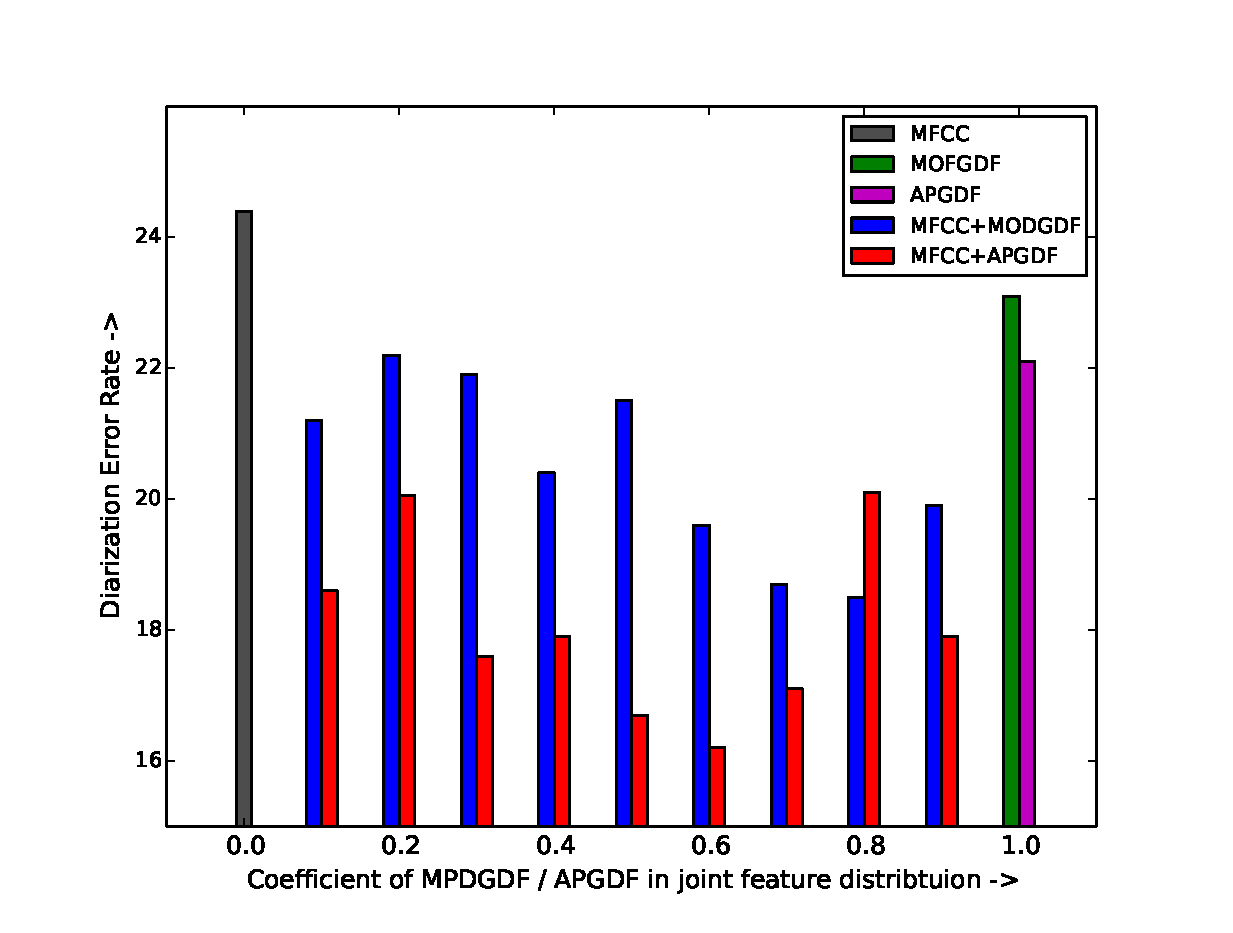
\includegraphics[width=0.5\textwidth,height=5.5cm]{figures/newFusionResults.eps}
\caption{Performance on AMI dataset comparing MFCC and its fusion with MODGDF
and APGDF with respect to weight of probabilities used for MODGDF and APGDF
features. Fusion weights are mentioned in parentheses.}
\label{fig:fusionResults}
\end{figure}
%\end{comment}

where $W_{m}$ and $W_{g}$ represents the weights of feature streams $m$ and $g$ 
such that $W_{m}$ + $W_{g}$ = $1$. In our case, feature $m$ is MFCC and feature 
$g$ is either of MODGDF or APGDF. Performance of various features and their fusion 
with respect to parameter $W_g$ is depicted in Fig. \ref{fig:fusionResults}. The fusion results 
show improvements in diarization error with increase in $W_g$, which indicates that group delay-based 
feature has value when used in supplement with MFCC features. However, furthermore increase in $W_g$ leads to deterioration of the overall performance the diarization system, as visible in Fig. \ref{fig:fusionResults}.   


%% Following paragraph is commented out, please ignore
%\begin{comment}
%The IB based diarization system are attractive to extended for multiple
%feature streams, due to fact that computational complexity with number of features streams. 
%One must notice that features are fused at the level of relevance variables,
%which allow to fuse probabilities instead of likelihoods, hence less affected by
%the number of dimensions of every feature stream (\cite{aIB}). Unfortunately, it
%introduces optimization of $W_i$ parameters, which is an computationally
%intensive task as for every new $W_i$ requires further optimization for
%parameters present in $p(y|x^{F_{i}},M^{F_{i}})$, e.g, $\beta$ of aIB.
%\end{comment}

\section{Experiments and Results }
\label{experimentsNresults}

The performance of the proposed group-delay based features for
speaker diarization is evaluated using publicly available AMI meeting corpus \cite{AMIData}. In
our experiments, we randomly select 100 meetings out of the total 170 meetings present in
the corpus. Further, data is divided into two sets, namely, development set ($30\%$) and test set ($70\%$).
The development set is used to obtain the optimal values of $\beta$ for aIB and in case of
feature fusion weights as well. And at last, the test set is utilized to asses the performance of various feature streams using optimal weights. The performance measure used in our experiments is Diarization error rate (DER) which can be defined as follows: 

\begin{equation}
DER = MISS + FA + SER
\end{equation}
\begin{comment}
\begin{equation}
	SER = \frac{\sum \limits_{s} {T_s ( min(N_{r}(s),N_{h}(s)) - N_{c}(s) ) } }  { \sum \limits_{s} T_s N_{r}(s)}
\end{equation}
\end{comment}

where MISS, FA and SER represents  missed speech, false alarm speech, and speaker error (for details on DER, see \cite{NIST}). The overlap speech is also included in calculation of the results, for all the experiments presented in this work. 

\begin{comment}
\begin{figure}[h]
\centering
\includegraphics[width=0.5\textwidth,height=5.5cm]{Images/devNtest.png}
\caption{Fusion results}
\label{fig:fusionResults}
\end{figure}
\end{comment}

\subsection{Feature extraction using MODGDF and APGDF}

We perform frame-blocking with $2/3$-overlapping windows of duration 30 ms and it remain same for all feature streams. While extracting MFCC features, the number of filters and the feature dimension were fixed to $40$ and $18$ respectively. The procedure used to compute MODGDF can be described as follows:

\begin{enumerate}
\item Compute the discrete Fourier transform for speech frame $X[n]$, and its time
multiplied version $Y[n]=nX[n]$.
\item Cepstrally smooth the $|X(\omega)|$ to estimate $|S(\omega)|$,
and then plug it into equation \ref{eq:MODGDF} to obtain $\tau_{m}(\omega)$.
\end{enumerate}	

\vspace{0.2cm}
Procedure to compute APGDF can be described as follows:
\begin{enumerate}
\item Perform all-pole analysis on speech frame $X[n]$ with prediction order set to
$p=20$, and estimate coefficients of all-pole filter, i.e., $a(k)$.  
\item Use G=1 and $a(k)$, to compute the frequency response $H(\omega)$ as defined
in equation \ref{eq:homega}.
\item Compute group delay function by taking the negative derivative of
the phase response of $H(\omega)$. Sample-wise
difference is used as an approximation to the derivative.
\end{enumerate}	
\vspace{0.2cm}

To extract feature from both MODGDF and APGDF, discrete cosine transform is applied, and the first $18$ coefficients (excluding the zeroth one) are utilized as the feature representation for further processing. Additional parameters involved in MODGDF, and APGDF computation ($\alpha =
0.9$, $\gamma=0.4$ and $p=20$) are directly taken from the earlier studies on speech
and speaker recognition \cite{modifiedGD,allPoleGdSid}. We do not perform search for the optimal value of these parameters as it requires computationally intensive experimentations, and the fact that the motivation of this work is to show the capability of group delay-based features and not to obtain the best performance. 

%\begin{comment}
\begin{table}[h]
\centering
\label{my-label}
\begin{tabular}{|l|l|l|}
\hline
Feature stream  & Development Set & Test Set \\ \hline
MFCC          & 24.4                   & 26.3            \\ \hline
MODGDF        & 23.1                   & 25.1            \\ \hline
APGDF         & 22.1                   & 24.9            \\ \hline
MFCC + MODGDF(0.8,0.2) & 18.5          & 20.1            \\ \hline
MFCC + APGDF(0.6,0.4)  & 16.2          & 18.7            \\ \hline
\end{tabular}
\vspace{0.4cm}
\label{table:results}
\caption{Diarization error obtained on AMI dataset comparing various feature
streams and their combinations. In case of fusion, optimum weights are mentioned
in parentheses.}
\end{table}
%\end{comment}


\subsection{Results}

Table \ref{table:results} presents the results of various feature streams and some of their
combinations for speaker diarization. The performance of MODGDF and APGDF
fairly indicates that group delay-based features have the ability to represent
speakers for IB based diarization system. The relative improvements
of $4.56\%$ and $5.32\%$ in DER are obtained by MODGDF and APGDF with respect to MFCC
respectively. The fusion of group delay based-features with MFCC and APGDF has also been
studied and results of these experiments are reported as MFCC + MODGDF and MFCC + APGDF in Table \ref{table:results} respectively. The results show that group delay-based features on fusion with MFCC have the potential to improve the performance of the current diarization systems, as the relative improvements of $23.5\%$ and $28.9\%$ by MFCC + MODGDF and MFCC + APGDF have been observed respectively.

The optimal fusion weights for MFCC + MODGDF and MFCC + APGDF are found (0.8,0.2) and
(0.6,0.4) respectively. We suspect that the relatively lesser improvements provided by
MODGDF when compared to APGDF, are due to fact that its computation critically depends on $\alpha$ and $\gamma$ parameters and search for their optimal values have been avoided. 
Results in Fig. \ref{fig:fusionResults} show that MODGDF or APGDF on fusion with MFCC outperforms any individual feature standalone, which suggests that these feature can supplement MFCC feature for IB based speaker diarization.

\section{Conclusion And Future Work}
\label{conclude}

In this work, we investigate the group-delay based features for IB based
diarization. Both with and without model based techniques, namely,
MODGDF and APGDF are used to estimate group-delay function and derive features for diarization. 
We found that features computed using MODGDF and APGDF provide better diarization error rate. 
Furthermore, these features has yielded a significant improvement in the diarization accuracy 
on fusion with MFCC. 

In future, it will be interesting to further investigate their ability in
more complex scenarios, e.g., for handling overlap speech and speech/non-speech
detection at early stage of a diarization system. Additionally, the fusion study of
other spectral and time domain features with group-delay based features appears
a reasonable direction to explore further. 

\bibliographystyle{IEEEbib}
\bibliography{bare_conf}

\end{document}


